\documentclass[11pt,a4paper]{article}

% =========================================================
% PACOTES ESSENCIAIS
% =========================================================
\usepackage[utf8]{inputenc}
\usepackage[T1]{fontenc}
\usepackage[brazilian]{babel}
\usepackage{geometry}
\usepackage{xcolor}
\usepackage{tabularx}
\usepackage{booktabs}
\usepackage{array}
\usepackage{enumitem}
\usepackage{helvet}
\usepackage{ragged2e}
\usepackage{fancyhdr}
\usepackage{lastpage}
\usepackage{url}
\usepackage{cite}
\usepackage{graphicx}
\usepackage{float}
\usepackage{caption}
\usepackage{subcaption}
\usepackage{microtype}
\usepackage[colorlinks=true,linkcolor=primary,citecolor=primary,urlcolor=primary]{hyperref}

% =========================================================
% CORES E ESTILO
% =========================================================
\definecolor{primary}{RGB}{20, 50, 100}
\definecolor{secondary}{RGB}{80, 90, 110}
\definecolor{accent}{RGB}{180, 40, 40}
\definecolor{lightgray}{RGB}{245, 247, 250}
\definecolor{bordergray}{RGB}{210, 215, 225}

\renewcommand{\familydefault}{\sfdefault}

\geometry{
  top=3.35cm,
  bottom=1.8cm,
  left=2.0cm,
  right=2.0cm,
  headheight=64pt,
  headsep=0.45cm
}

\setlength{\parindent}{0pt}
\setlength{\parskip}{0.55em}
\setlist[itemize]{leftmargin=1.5em, itemsep=0.2em}
\setlist[enumerate]{leftmargin=1.5em, itemsep=0.2em}

\newcolumntype{Y}{>{\centering\arraybackslash}X}
\newcolumntype{L}{>{\raggedright\arraybackslash}X}

\AtEndDocument{\label{LastPage}}

% =========================================================
% CAMPOS DO DOCUMENTO
% =========================================================
\newcommand{\NomeProjeto}{Mapa de Calor e Predição do Risco de Acidentes de Trânsito na BR-230}
\newcommand{\VersaoModelo}{1.0}
\newcommand{\DataEmissao}{03/11/2026}

\newcommand{\IntegranteTres}{Winy Gabrielly Soares de Oliveira}
\newcommand{\IntegranteDois}{Ricardo Diniz Mendes}
\newcommand{\IntegranteUm}{João Batista Santos Silva Neto}

\newcommand{\Componentes}{
João Batista Santos Silva Neto \\
Ricardo Diniz Mendes \\
Winy Gabrielly Soares de Oliveira
}

\newcommand{\EmailTres}{winy.soares@discente.ufma.br}
\newcommand{\EmailDois}{ricardo.dm@discente.ufma.br}
\newcommand{\EmailUm}{jbss.neto@discente.ufma.br}

% =========================================================
% CABEÇALHO
% =========================================================
\newcommand{\CabecalhoProjeto}{%
\begin{minipage}{\textwidth}
\centering
\renewcommand{\arraystretch}{1.25}

\begin{tabularx}{\textwidth}{|p{2.0cm}|X|p{4.2cm}|}
\hline
& \centering\textbf{Documentação do Projeto}\arraybackslash
& Versão do Modelo: \VersaoModelo \\
\cline{3-3}
& &
Emissão: \DataEmissao
\quad Página: \thepage/\pageref{LastPage} \\
\cline{2-3}
&
\multicolumn{2}{l|}{
Projeto:
\hfill
\textbf{\NomeProjeto}
\hfill
} \\
\hline
\end{tabularx}

\end{minipage}%
}

\pagestyle{fancy}
\fancyhf{}
\fancyhead[C]{\CabecalhoProjeto}
\renewcommand{\headrulewidth}{0pt}
\renewcommand{\footrulewidth}{0pt}

\makeatletter
\renewcommand\section{
\@startsection{section}{1}{0pt}%
{1.4ex plus .2ex minus .2ex}%
{0.8ex plus .2ex}%
{\normalfont\Large\bfseries\color{primary}}
}
\renewcommand\subsection{
\@startsection{subsection}{2}{0pt}%
{1.2ex plus .2ex minus .2ex}%
{0.6ex plus .2ex}%
{\normalfont\large\bfseries\color{secondary}}
}
\renewcommand\subsubsection{
\@startsection{subsubsection}{3}{0pt}%
{1.0ex plus .2ex minus .2ex}%
{0.5ex plus .2ex}%
{\normalfont\normalsize\bfseries}
}
\makeatother

\begin{document}

% ---------------------------------------------------------
% CAPA
% ---------------------------------------------------------
\begin{center}
\vspace*{1.2cm}

{\Large\textbf{Projeto da Disciplina Ciência de Dados}}\\[0.8em]

{\Large\textbf{Fase 3: Preparação dos Dados (CRISP-DM)}}

\end{center}

\vspace{0.8cm}
\vfill

\begin{center}

{\Huge\textbf{Relatório de Formatação, Seleção, Limpeza, Construção e Integração}}\\[1.5cm]

{\Large\Componentes}\\[1.5cm]

{\Large\textbf{\NomeProjeto}}\\[0.5cm]

\textit{Universidade Federal do Maranhão (UFMA) \\ Programa de Pós-Graduação em Ciência da Computação (PPGCC)}

\end{center}

\vfill
\newpage

% ---------------------------------------------------------
% HISTÓRICO
% ---------------------------------------------------------
\section*{Histórico de Revisões do Documento}

\vspace{0.6em}

\begin{center}
\renewcommand{\arraystretch}{1.35}

\begin{tabularx}{\textwidth}{|p{1.6cm}|X|p{3.2cm}|p{2.8cm}|p{2.2cm}|}
\hline
\textbf{Revisão} & \textbf{Descrição} & \textbf{Modificado por} & \textbf{Status} & \textbf{Data} \\
\hline
1.0 &
Elaboração do Relatório da Fase de Preparação dos Dados a partir da matriz de encaminhamentos da Fase~2: base BR-230 2022--2025, limpezas, atributos derivados, partição prospectiva e artefatos em \texttt{bases/preparadas/}. &
Equipe do projeto &
Concluído &
03/11/2026 \\
\hline
\end{tabularx}
\end{center}

\newpage

% =========================================================
% 1 INTRODUÇÃO
% =========================================================
\section{Introdução e Objetivo da Fase}

A Fase~3 do CRISP-DM (\textit{Data Preparation}) transforma dados brutos em um conjunto pronto para mineração~\cite{chapman2000}. No guia clássico, essa etapa concentra a maior parte do esforço do projeto e compreende cinco tarefas: \textbf{formatar}, \textbf{selecionar}, \textbf{limpar}, \textbf{construir} e \textbf{integrar}.

No projeto da BR-230, o objetivo de negócio permanece o definido na Fase~1: combinar mapa de calor da concentração histórica de acidentes com um componente preditivo de risco~\cite{santos2021,behboudi2024}. A Fase~2 fechou o diagnóstico com 6.217 ocorrências pós-pandemia (2022--2025), variável-alvo ``Com Vítimas Fatais'' (603 casos; 9,70\%) e uma matriz explícita de decisões para a preparação.

Este relatório documenta a execução dessa matriz no notebook \texttt{preparacao\_dos\_dados.ipynb}, alinhada a operações do \textit{Data Wrangling with pandas Cheat Sheet} (\texttt{concat}, \texttt{query}, \texttt{merge}, \texttt{groupby}/\texttt{agg}, seleção de colunas e encadeamento de transformações).

\subsection{Escopo e produtos}

\begin{itemize}
    \item Universo: arquivos \texttt{datatran2022.csv} a \texttt{datatran2025.csv} e \texttt{acidentes2022.csv} a \texttt{acidentes2025.csv} da PRF~\cite{prfdados}.
    \item Grão analítico principal: \textbf{1 linha = 1 ocorrência} na BR-230.
    \item Produtos: base limpa completa; conjunto de modelagem com preditores contextuais; partição treino (2022--2024) / teste (2025); figura de controle.
\end{itemize}

A modelagem estima a probabilidade condicional $P(\text{Fatal} \mid \text{Acidente}, \text{contexto})$. A base da PRF não traz Volume Médio Diário; o mapa de calor continua expressando densidade histórica de ocorrência, não exposição ao tráfego.

\newpage

% =========================================================
% 2 FORMATAÇÃO
% =========================================================
\section{Formatação dos Dados}

A tarefa \textit{Format data} ajusta a sintaxe dos arquivos sem alterar o significado analítico.

\subsection{Codificação, delimitadores e tipos}

Os CSV da PRF estão em \texttt{ISO-8859-1} (\textit{latin-1}), usam ponto e vírgula como separador de campos e vírgula como separador decimal. A rotina de carga fixa \texttt{encoding='latin-1'}, \texttt{sep=';'} e \texttt{decimal=','}, garantindo que latitude, longitude e quilômetro entrem como \texttt{float64}.

Em seguida:
\begin{itemize}
    \item nomes de coluna são normalizados para minúsculas;
    \item \texttt{data\_inversa} e \texttt{horario} geram \texttt{data}, \texttt{hora}, \texttt{ano} e \texttt{mes};
    \item contagens de pessoas e veículos são forçadas a numérico com \texttt{errors='coerce'}.
\end{itemize}

Essa formatação é pré-condição da espacialização (WGS84) e da partição temporal prospectiva.

\subsection{Reprodutibilidade da ingestão}

Se um arquivo não existir em \texttt{bases/}, a função \texttt{garantir\_base()} baixa o ZIP oficial do Google Drive da PRF e extrai o CSV. Em redes com inspeção HTTPS, o cliente HTTP combina o bundle do \texttt{certifi} com as autoridades do chaveiro do sistema, preservando a verificação de certificado.

\newpage

% =========================================================
% 3 SELEÇÃO E INTEGRAÇÃO
% =========================================================
\section{Seleção e Integração}

\subsection{Integração temporal das ocorrências}

Os quatro anos de \texttt{datatran} são empilhados com \texttt{pd.concat} (união vertical de observações). O recorte viário usa \texttt{query("br == 230")}. A Tabela~\ref{tab:volume_prep} confirma a série já descrita na Fase~2.

\begin{table}[H]
\centering
\small
\renewcommand{\arraystretch}{1.2}
\caption{Volume consolidado da BR-230 após integração temporal (ocorrências).}
\label{tab:volume_prep}
\begin{tabularx}{\textwidth}{|c|c|c|c|c|}
\hline
\textbf{Ano} & \textbf{Acidentes} & \textbf{Fatais} & \textbf{Mortos} & \textbf{Prop. fatal (\%)} \\
\hline
2022 & 1.345 & 135 & 148 & 10,04 \\
\hline
2023 & 1.403 & 143 & 160 & 10,19 \\
\hline
2024 & 1.724 & 157 & 175 & 9,11 \\
\hline
2025 & 1.745 & 168 & 192 & 9,63 \\
\hline
\textbf{Total} & \textbf{6.217} & \textbf{603} & \textbf{675} & \textbf{9,70} \\
\hline
\end{tabularx}
\end{table}

\subsection{Seleção de atributos por papel analítico}

A Tabela~\ref{tab:papeis} separa atributos de contexto (preditores), desfecho e campos de auditoria. A seleção evita vazamento: contagens de vítimas e a própria classificação não entram como entrada do classificador. \texttt{causa\_acidente} e \texttt{tipo\_acidente} permanecem no arquivo completo, mas fora do conjunto principal de preditores, porque a Fase~2 registrou que são preenchidos após a ocorrência.

\begin{table}[H]
\centering
\small
\renewcommand{\arraystretch}{1.25}
\caption{Papéis dos atributos no conjunto preparado.}
\label{tab:papeis}
\begin{tabularx}{\textwidth}{|p{3.2cm}|X|p{3.6cm}|}
\hline
\textbf{Papel} & \textbf{Exemplos} & \textbf{Destino} \\
\hline
Contexto (preditores) &
UF, município, km, latitude, longitude, dia da semana, hora, mês, fase do dia, clima, tipo de pista, traçado principal, uso do solo, sentido, flags derivados e agregados de pessoa &
Modelo e mapa \\
\hline
Desfecho &
\texttt{alvo\_fatal}, \texttt{classificacao\_acidente}, \texttt{mortos}, \texttt{feridos} &
Alvo / auditoria \\
\hline
Auditoria / exploração &
Traçado original, divergência UF$\times$regional, km acima do DNIT, causa e tipo &
Arquivo completo \\
\hline
\end{tabularx}
\end{table}

\subsection{Integração com o arquivo por pessoa}

Os arquivos \texttt{acidentesYYYY.csv} (15.764 linhas na BR-230) são agregados por \texttt{id} do acidente e unidos à base de ocorrências com \texttt{merge} (\textit{left join}, validação um-para-um). A agregação produz:
\begin{itemize}
    \item \texttt{tem\_motocicleta} (3.244 acidentes com ao menos uma motocicleta);
    \item \texttt{tem\_pedestre} (270);
    \item \texttt{idade\_media} (239 acidentes sem idade válida após conversão de sentinelas, 3,8\%).
\end{itemize}
Todos os 6.217 acidentes encontram ao menos uma linha de pessoa correspondente. O grão de ocorrência não é inflado.

\newpage

% =========================================================
% 4 LIMPEZA
% =========================================================
\section{Limpeza dos Dados}

A Tabela~\ref{tab:limpeza} resume as checagens executadas sobre a série consolidada.

\begin{table}[H]
\centering
\small
\renewcommand{\arraystretch}{1.2}
\caption{Resultado das limpezas e sinalizações na BR-230 (2022--2025).}
\label{tab:limpeza}
\begin{tabularx}{\textwidth}{|p{6.2cm}|c|X|}
\hline
\textbf{Checagem} & \textbf{Quantidade} & \textbf{Tratamento} \\
\hline
Acidentes no recorte & 6.217 & Base única de ocorrências \\
\hline
Alvo positivo (\texttt{alvo\_fatal}=1) & 603 (9,70\%) & Variável-alvo binária \\
\hline
Traçados compostos (\texttt{;}) & 1.606 & Redução a \texttt{tracado\_principal} + flag \\
\hline
UF do município $\neq$ UF da regional & 109 & Prevalecem UF e coordenadas do local \\
\hline
km acima do limite DNIT (TO) & 1 & \texttt{km\_ajustado}=144,7; original preservado \\
\hline
Rural + pista simples & 1.840 & Flag de combinação crítica \\
\hline
Rural + simples fora da Paraíba & 1.040 (25,1\% fatais) & Flag \texttt{fora\_pb} \\
\hline
\texttt{pesid}=0 convertido a nulo & 876 linhas de pessoa & Sentinela $\rightarrow$ \texttt{NaN} \\
\hline
\end{tabularx}
\end{table}

\subsection{Variável-alvo}

Define-se
\[
\texttt{alvo\_fatal} =
\begin{cases}
1, & \text{se }\texttt{classificacao\_acidente}=\text{``Com Vítimas Fatais''},\\
0, & \text{caso contrário.}
\end{cases}
\]
A construção é determinística a partir do rótulo oficial da PRF e coincide com os 603 sinistros fatais da Fase~2.

\subsection{Traçado composto}

Em 1.606 registros, \texttt{tracado\_via} contém mais de um valor separado por ponto e vírgula. A preparação cria \texttt{tracado\_principal} (primeiro valor) e a flag \texttt{tracado\_composto}, permitindo tanto a modelagem com cardinalidade reduzida quanto auditoria do campo original.

\subsection{Prevalência geográfica e marco do Tocantins}

Nas 109 divergências entre a UF do município e a UF embutida em \texttt{regional}, prevalecem a UF e as coordenadas do local do sinistro, conforme a Fase~2. No Tocantins, um registro com km 146,0 ultrapassa os 144,7~km publicados pelo DNIT~\cite{dnit2026}; \texttt{km\_ajustado} recebe o teto cadastral sem descartar a ocorrência.

\subsection{Completude operacional dos preditores contextuais}

Latitude, longitude, km, fase do dia, clima, pista, uso do solo e demais preditores categóricos de ocorrência estão integralmente preenchidos nas 6.217 linhas. O único atributo contextual com omissão relevante no conjunto de modelagem é \texttt{idade\_media} (239 nulos), herdado das idades sentinela do arquivo por pessoa.

\newpage

% =========================================================
% 5 CONSTRUÇÃO
% =========================================================
\section{Construção de Atributos e Partição}

\subsection{Atributos derivados}

Além do alvo e do traçado principal, foram construídos:
\begin{itemize}
    \item \texttt{area\_urbana} / \texttt{area\_rural} a partir de \texttt{uso\_solo};
    \item \texttt{fim\_de\_semana} a partir do dia da semana normalizado;
    \item \texttt{periodo\_noturno} a partir de \texttt{fase\_dia};
    \item \texttt{rural\_pista\_simples} e \texttt{fora\_pb}, que materializam o achado de gravidade da Fase~2.
\end{itemize}

A Figura~\ref{fig:controle_prep} mostra o controle anual de volume versus proporção fatal e a letalidade por tipo de pista após a preparação.

\begin{figure}[H]
\centering
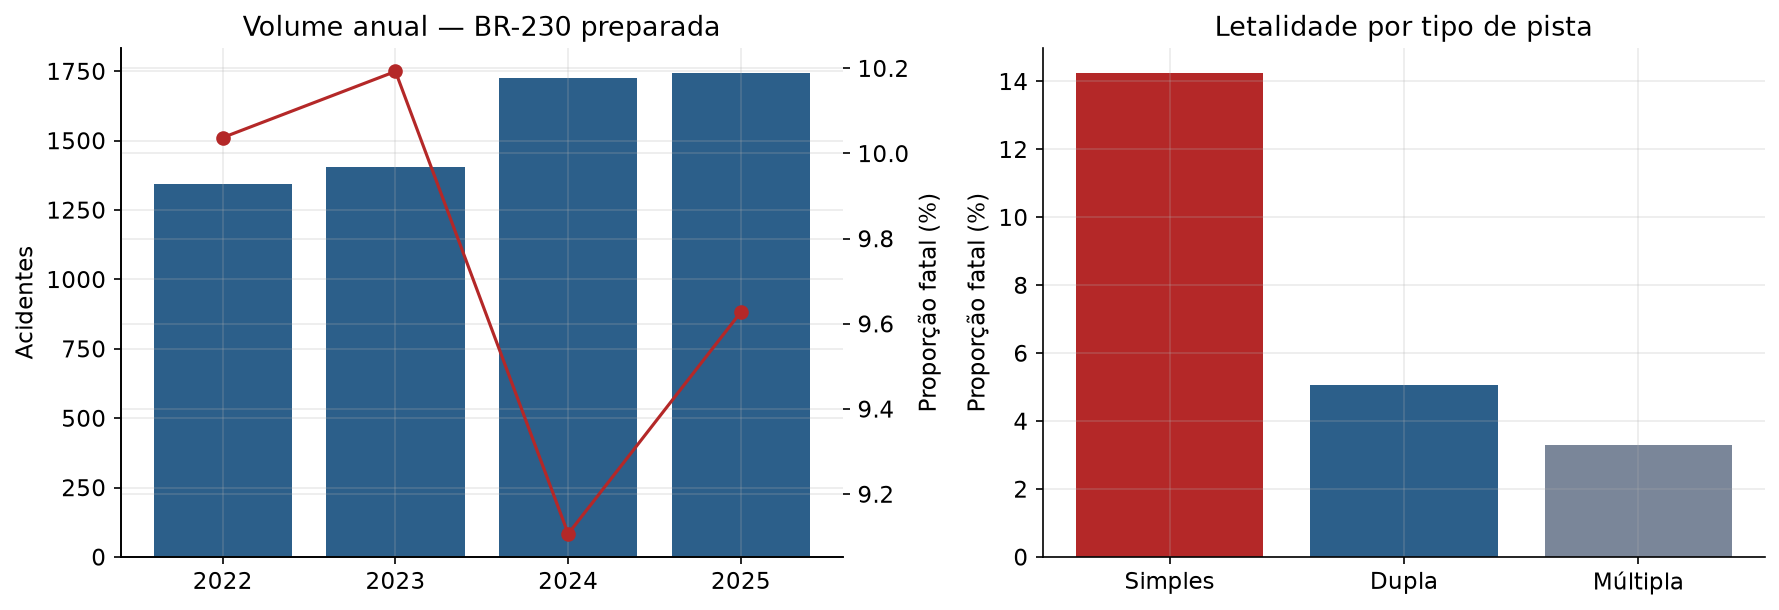
\includegraphics[width=0.95\textwidth]{figuras/preparacao_controle_anual_pista.png}
\caption{Controle da base preparada: volume e proporção fatal por ano (esquerda) e proporção fatal por tipo de pista (direita) na BR-230 (2022--2025).}
\label{fig:controle_prep}
\end{figure}

\subsection{Partição prospectiva treino/teste}

A divisão é temporal, não aleatória: treino em 2022--2024 e teste em 2025. A escolha preserva o papel de 2025 como horizonte prospectivo e como ano validado contra o Anuário Estatístico da PRF na Fase~2~\cite{prfanuario2025}.

\begin{table}[H]
\centering
\small
\renewcommand{\arraystretch}{1.2}
\caption{Partição prospectiva do conjunto de modelagem.}
\label{tab:particao}
\begin{tabularx}{\textwidth}{|l|c|c|c|}
\hline
\textbf{Conjunto} & \textbf{Acidentes} & \textbf{Fatais} & \textbf{Prop. fatal (\%)} \\
\hline
Treino (2022--2024) & 4.472 & 435 & 9,73 \\
\hline
Teste (2025) & 1.745 & 168 & 9,63 \\
\hline
\textbf{Total} & \textbf{6.217} & \textbf{603} & \textbf{9,70} \\
\hline
\end{tabularx}
\end{table}

O desbalanceamento (cerca de 1 caso fatal para 9,3 ocorrências) não é artificialmente equilibrado nesta fase. A Fase~4 deverá tratar ponderação de classes, limiar de decisão e métricas alinhadas aos critérios da Fase~1 (recall, precisão, F1, ROC-AUC e taxa de falsos negativos).

\newpage

% =========================================================
% 6 ARTEFATOS
% =========================================================
\section{Artefatos Gerados}

Os arquivos finais estão em \texttt{bases/preparadas/}, em CSV UTF-8 com vírgula.

\begin{table}[H]
\centering
\small
\renewcommand{\arraystretch}{1.25}
\caption{Inventário dos artefatos da Preparação dos Dados.}
\label{tab:artefatos}
\begin{tabularx}{\textwidth}{|p{5.4cm}|c|X|}
\hline
\textbf{Arquivo} & \textbf{Linhas} & \textbf{Conteúdo} \\
\hline
\texttt{br230\_ocorrencias\_preparadas.csv} & 6.217 & Base completa limpa (contexto, desfecho, auditoria e agregados de pessoa). \\
\hline
\texttt{br230\_modelo\_completo.csv} & 6.217 & Preditores contextuais + \texttt{alvo\_fatal}. \\
\hline
\texttt{br230\_modelo\_treino.csv} & 4.472 & Partição 2022--2024. \\
\hline
\texttt{br230\_modelo\_teste.csv} & 1.745 & Partição 2025. \\
\hline
\end{tabularx}
\end{table}

O notebook \texttt{preparacao\_dos\_dados/preparacao\_dos\_dados.ipynb} reproduz integralmente o pipeline. A figura de controle é salva em \texttt{preparacao\_dos\_dados/figuras/}.

\newpage

% =========================================================
% 7 ENCAMINHAMENTOS
% =========================================================
\section{Encaminhamentos para a Fase 4 (Modelagem)}

\begin{enumerate}
    \item Treinar o classificador binário de gravidade sobre \texttt{br230\_modelo\_treino.csv}, avaliando em \texttt{br230\_modelo\_teste.csv}.
    \item Usar apenas preditores contextuais; manter causa/tipo e contagens de vítimas fora da entrada do modelo principal.
    \item Tratar o desbalanceamento com pesos de classe e/ou ajuste de limiar, priorizando recall e baixa taxa de falso negativo, conforme as metas da Fase~1.
    \item Imputar ou isolar \texttt{idade\_media} nula (3,8\%) antes do treino, se o atributo for mantido.
    \item Construir o mapa de calor a partir de latitude/longitude da base preparada completa, podendo colorir pela probabilidade predita ou pela flag \texttt{alvo\_fatal}.
    \item Documentar a ausência de VMD: o produto preditivo expressa risco condicional à ocorrência registrada, não taxa por veículo-km.
\end{enumerate}

A Tabela~\ref{tab:rastreio} rastreia o cumprimento da matriz de decisões da Fase~2.

\begin{table}[H]
\centering
\small
\renewcommand{\arraystretch}{1.25}
\caption{Rastreio da matriz de decisões da Fase~2 na Preparação.}
\label{tab:rastreio}
\begin{tabularx}{\textwidth}{|p{4.4cm}|c|X|}
\hline
\textbf{Decisão da Fase~2} & \textbf{Status} & \textbf{Implementação} \\
\hline
Base única de ocorrências + partição 2022--2024 / 2025 & Cumprida & \texttt{concat} + \texttt{query} por ano \\
\hline
Posicionamento por coordenadas WGS84 & Cumprida & latitude/longitude numéricas, 0 nulos \\
\hline
Zeros sentinela $\rightarrow$ \texttt{NaN} & Cumprida & \texttt{pesid}, idade (e idade $>$100) \\
\hline
Traçado composto & Cumprida & primeiro valor + flag \\
\hline
Prevalência geográfica e km do TO & Cumprida & flags + \texttt{km\_ajustado} \\
\hline
Desbalanceamento documentado & Cumprida & 9,70\% no total; tratamento na Fase~4 \\
\hline
\end{tabularx}
\end{table}

\newpage

% =========================================================
% 8 REFERÊNCIAS
% =========================================================
\begin{thebibliography}{99}

\bibitem{chapman2000}
P.~Chapman, J.~Clinton, R.~Kerber, T.~Khabaza, T.~Reinartz, C.~Shearer e R.~Wirth.
\newblock \emph{{CRISP-DM} 1.0: Step-by-step data mining guide}.
\newblock CRISP-DM Consortium, 2000.
\newblock Dispon{\'i}vel em: \url{https://www.datascienceprocess.com/wp-content/uploads/2020/05/crisp-dm-guide.pdf}.

\bibitem{prfdados}
Pol{\'i}cia Rodovi{\'a}ria Federal.
\newblock Dados Abertos da {PRF} -- Acidentes de Tr{\'a}nsito.
\newblock Portal gov.br, acesso em 13/10/2026.
\newblock Dispon{\'i}vel em: \url{https://www.gov.br/prf/pt-br/acesso-a-informacao/dados-abertos/dados-abertos-da-prf}.

\bibitem{prfanuario2025}
Pol{\'i}cia Rodovi{\'a}ria Federal.
\newblock Anu{\'a}rio Estat{\'i}stico 2025 da Pol{\'i}cia Rodovi{\'a}ria Federal.
\newblock Divulgado em Maio de 2026.
\newblock Dispon{\'i}vel em: \url{https://www.gov.br/prf/pt-br/noticias/nacionais/2026/maio/prf-divulga-anuario-estatistico-de-2025-com-aumento-de-infracoes-e-reducao-de-mortes-nas-rodovias-federais}.

\bibitem{dnit2026}
Departamento Nacional de Infraestrutura de Transportes ({DNIT}).
\newblock Restaura{\c{c}}{\~a}o e Extens{\~o}es da Rodovia {BR-230}.
\newblock Portal gov.br/dnit, 2026.
\newblock Dispon{\'i}vel em: \url{https://www.gov.br/dnit/pt-br}.

\bibitem{tozetto2025}
J.~P.~Tozetto, I.~Nunes, B.~Soares, E.~T.~Albergaria, D.~R.~C.~Dias, V.~F.~S.~Mota e L.~C.~D.~Rocha.
\newblock Evaluating Segmentation and Temporal Resolution in Highway Crash Forecasting: The {BR-040} Corridor.
\newblock In \emph{Springer} (cap{\'i}tulo de livro), 2025.
\newblock DOI: \url{https://doi.org/10.1007/978-3-032-30488-9_36}.

\bibitem{santos2021}
D.~Santos, J.~Saias, P.~Quaresma e V.~B.~Nogueira.
\newblock Machine Learning Approaches to Traffic Accident Analysis and Hotspot Prediction.
\newblock \emph{Computers}, 10(12):157, 2021.
\newblock DOI: \url{https://doi.org/10.3390/computers10120157}.

\bibitem{behboudi2024}
N.~Behboudi, S.~Moosavi e R.~Ramnath.
\newblock Recent Advances in Traffic Accident Analysis and Prediction: A Comprehensive Review of Machine Learning Techniques.
\newblock \emph{arXiv preprint} arXiv:2406.13968, 2024.
\newblock Dispon{\'i}vel em: \url{https://arxiv.org/abs/2406.13968}.

\bibitem{le2020}
K.~G.~Le, P.~Liu e L.-T.~Lin.
\newblock Traffic accident hotspot identification by integrating kernel density estimation and spatial autocorrelation analysis: a case study.
\newblock \emph{International Journal of Crashworthiness}, 27(2):543--553, 2022.
\newblock DOI: \url{https://doi.org/10.1080/13588265.2020.1826800}.

\bibitem{iranmanesh2022}
M.~Iranmanesh, S.~Seyedabrishami e S.~Moridpour.
\newblock Identifying high crash risk segments in rural roads using ensemble decision tree-based models.
\newblock \emph{Scientific Reports}, 12:21324, 2022.
\newblock DOI: \url{https://doi.org/10.1038/s41598-022-24476-z}.

\bibitem{gao2024}
X.~Gao, X.~Jiang, J.~Haworth, D.~Zhuang, S.~Wang, H.~Chen e S.~Law.
\newblock Uncertainty-aware probabilistic graph neural networks for road-level traffic crash prediction.
\newblock \emph{Accident Analysis \& Prevention}, 208:107801, 2024.
\newblock DOI: \url{https://doi.org/10.1016/j.aap.2024.107801}.

\bibitem{khan2024}
A.~A.~Khan e J.~Hussain.
\newblock Utilizing {GIS} and Machine Learning for Traffic Accident Prediction in Urban Environment.
\newblock \emph{Civil Engineering Journal}, 10(6):1922--1935, 2024.
\newblock DOI: \url{https://doi.org/10.28991/CEJ-2024-010-06-013}.

\bibitem{he2025}
M.~He, G.~Meng, X.~Wu, X.~Han e J.~Fan.
\newblock Road Traffic Accident Prediction Based on Multi-Source Data -- A Systematic Review.
\newblock \emph{Promet -- Traffic\&Transportation}, 37(2):499--522, 2025.
\newblock DOI: \url{https://doi.org/10.7307/ptt.v37i2.763}.

\bibitem{jeyabharathi2026}
J.~Jeyabharathi, K.~J.~Lakshmi Prasad, K.~Karunakar, K.~Sai Charan e R.~Sasi Preetham.
\newblock {AI}-Driven Traffic Accident Prediction: Integrating Real-Time Weather, Analytics, and Machine Learning for Enhanced Road Safety.
\newblock In \emph{2026 9th International Conference on Intelligent Computing and Control Systems (ICICCS)}, p.~799--804, 2026.
\newblock DOI: \url{https://doi.org/10.1109/ICICCS67901.2026.11502769}.

\bibitem{affou2026}
H.~Affou, D.~Teso-Fz-Beto{\~n}o, U.~Fernandez-Gamiz, J.~A.~Ramos-Hernanz, D.~Caballero-Martin e J.~M.~Lopez-Guede.
\newblock Advances in Traffic Accident Prediction: A Survey of Novel Approaches.
\newblock \emph{Urban Science}, 10(7):349, 2026.
\newblock DOI: \url{https://doi.org/10.3390/urbansci10070349}.

\end{thebibliography}


\end{document}
